\chapter{Experiments and Evaluation}
\label{cha:experiments}

This chapter presents the experimental setup, training process, and evaluation of the ControlNet integration into MESA for steerable terrain generation. The experiments were designed to assess the impact of different training variants on the model's ability to learn spatial conditioning and to evaluate the quality and alignment of the generated landscapes with the provided control maps.

\section{Training Variants}
\label{sec:training_variants}

There are several key training variants explored in this thesis, each designed to investigate different aspects of conditioning and optimization for the ControlNet architecture. The primary variants include:

\begin{itemize}
	\item \textbf{Guided Hints:} Standard ControlNet injects the first conditioning into the single UNet decoder head, which is used to condition on the control maps. As MESA has two separate Heads it raised the question of whether one shared hint suffices or whether separate hints per head yield better feature alignment.
	\item \textbf{SNR Weighting:} Implementing a Signal-to-Noise Ratio (SNR) weighting scheme in the loss function to prioritize learning at different noise levels during the diffusion process.
	\item \textbf{Optimizers:} Evaluating different optimization algorithms, including Prodigy, Adam, and Adam8bit.
	\item \textbf{Precision:} Comparing training with bf16 versus fp16 precision to understand the trade-offs between memory efficiency and numerical stability in the context of ControlNet training.
\end{itemize}

\section{Overfit Experiments}
\label{sec:overfit_experiments}

To keep the training runs manageable, most experiments were conducted on a small subset of the data first to test for training stability and convergence. This included overfitting on a single sample or a small batch of samples to ensure that the model can learn to reproduce the conditioning maps accurately before scaling up to the full dataset. These preliminary experiments were crucial for debugging the training pipeline, validating the implementation of the ControlNet architecture, and doing a preliminary assessment of different training variants. The model showed the ability to overfit on reduced data, with SNR weighting and separate hints per head showing promising results in terms of faster convergence and better alignment with the conditioning maps. In terms of optimizers, Prodigy demonstrated roughly comparable perfomance to tuned Adam. The precision comparison revealed that fp16 converges better than bf16 in this context.

\section{Full Training Run}
\label{sec:final_training_run}

The full training run was conducted using the SNR-weighted loss function, the Prodigy optimizer, and the configuration with two separate guided hints for each head. The training was performed for a total of $16\,000$ steps on the MajorTOM~\cite{schulz2024majortom} dataset, with periodic evaluation of the mean Intersection over Union every $1\,000$ steps. The training metrics, shown in Figure~\ref{fig:training_metrics}, indicate a significant breakthrough in mIoU around steps $8\,000$ to $10\,000$, where the model begins to effectively learn the conditioning maps. However, after this initial improvement, the mIoU exhibits random fluctuations, suggesting that while the model has learned to some extent, it may still be struggling with consistent generalization. The norms of the ControlNet residual outputs per block show an increasing influence of the control signal over time, with noticeable breakouts at steps $11\,000$ and $15\,000$, which were caused by an accumulation bug with the loggign in connection to run restarts. The bucket loss and total loss metrics are too noisy to interpret clearly, as they fluctuate around the same level throughout the training process, indicating that they may not be reliable indicators of training progress in this context.

\begin{figure}[htbp]
	\centering
	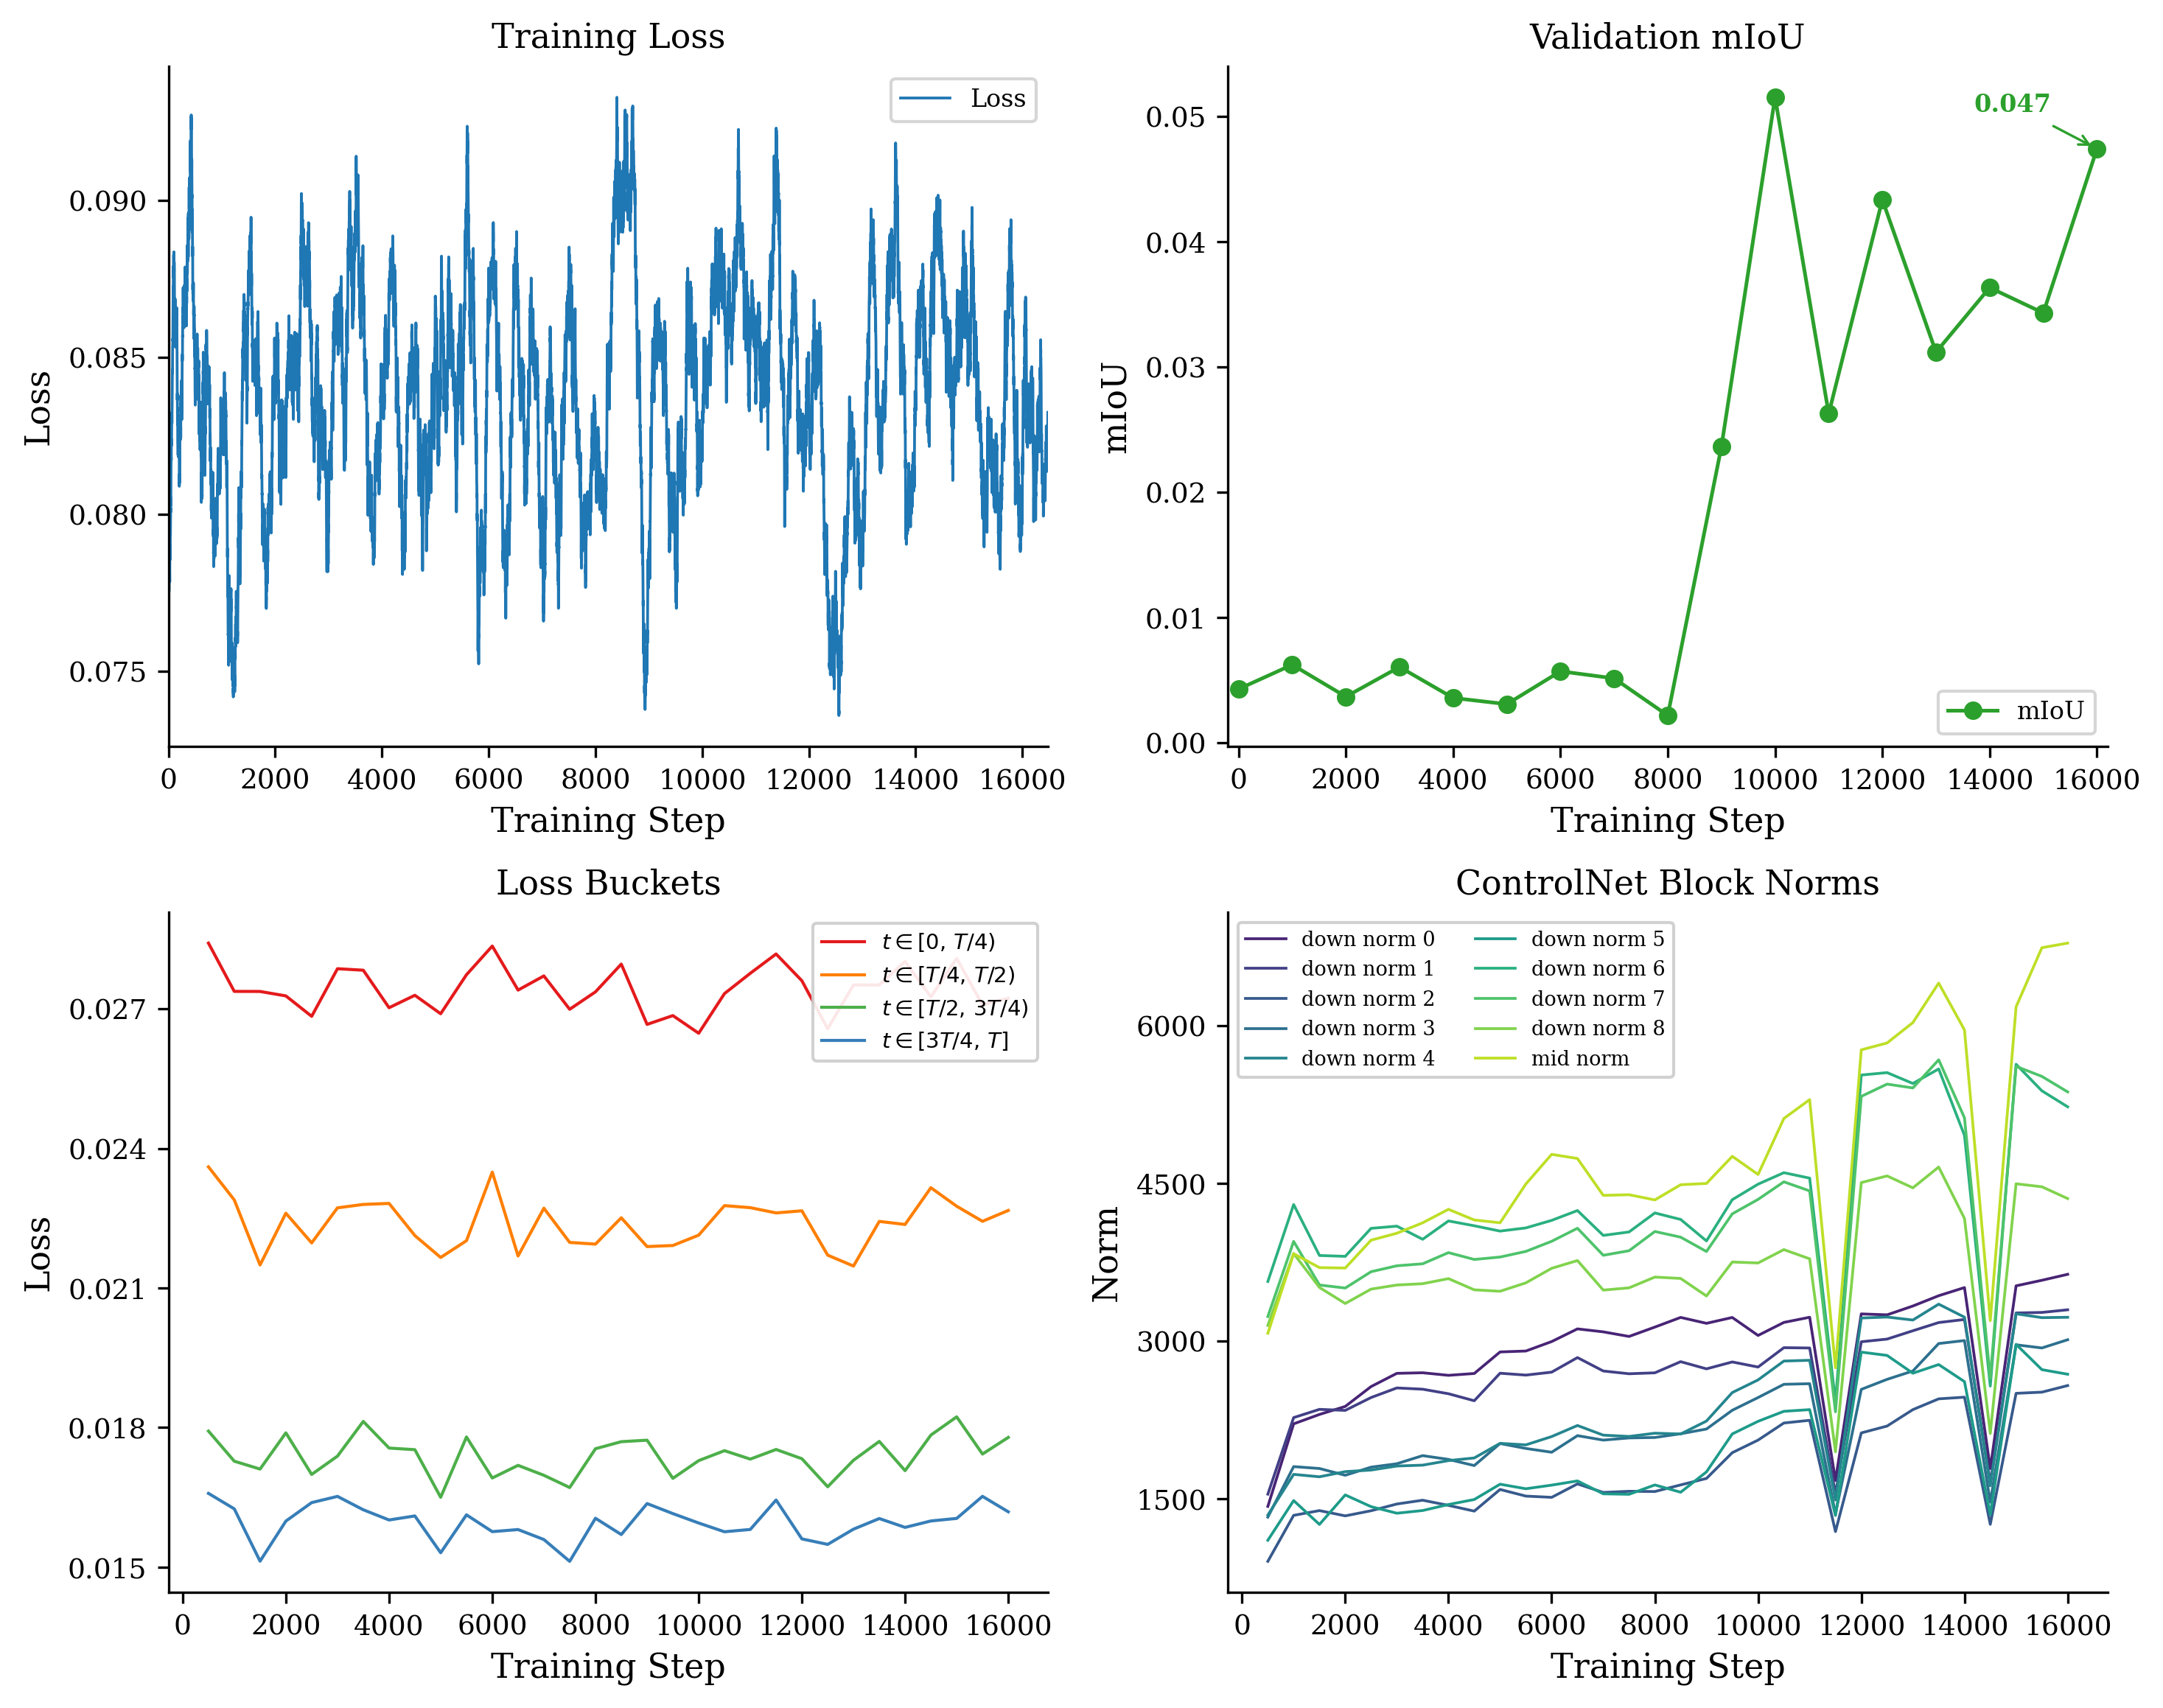
\includegraphics[width=\linewidth]{images/training_metrics.png}
	\caption{Training metrics for the training run. \textbf{Top-left:} training loss with a 200-step rolling average. \textbf{Top-right:} validation mean Intersection over Union evaluated every 1\,000 steps. \textbf{Bottom-left:} per-bucket loss decomposed by noise level ($t/4$ quantiles). \textbf{Bottom-right:} norms of the ControlNet residual outputs per block.}
	\label{fig:training_metrics}
\end{figure}

\subsection{Baseline Comparisons}
\label{sec:baseline_comparisons}

The control weighting sweep, shown in Figure~\ref{fig:control_weight_sweep}, demonstrates the effect of varying the conditioning scale $w$ on the generated terrain. All images were produced with the same random seed ($42$), the same text prompt (\enquote{A Sentinel-2 image of subpolar forests and mountains in Chile in January}), and the same ridge/valley/cliff control map. As $w$ increases the generated landscape progressively conforms to the spatial structure.

\begin{figure}[htbp]
	\centering
	\includegraphics[width=\linewidth]{images/control_weight_sweep.png}
	\caption{Control weight sweep demonstrating the effect of varying the conditioning scale $w$ on the generated terrain.}
	\label{fig:control_weight_sweep}
\end{figure}

\subsection{Quantitative Evaluation}
\label{sec:quantitative_evaluation}

The quantitative evaluation of the generated landscapes was conducted by calculating the Intersection over Union between the extracted terrain features from the generated Digital Elevation Models and the original conditioning maps. The distribution of IoU scores across 100 generated terrain samples with a control weight of $w = 1.4$ is shown in Figure~\ref{fig:iou_distribution}. The results indicate that valleys achieve the highest alignment with the conditioning maps, with a mIoU of $0.117$, while cliffs show the lowest alignment, with a mean IoU of $0.0$. The variance of IoU scores is quite high for all channels, which could be attributed to the model being undertrained or potentially due to a more general issue in methodology especially in conjunction with the observed flattening of the generated landscapes at higher control weights. It could also be due to the sparsity of the feature maps which makes the IoU metric very sensitive to small misalignments.

\begin{figure}[htbp]
	\centering
	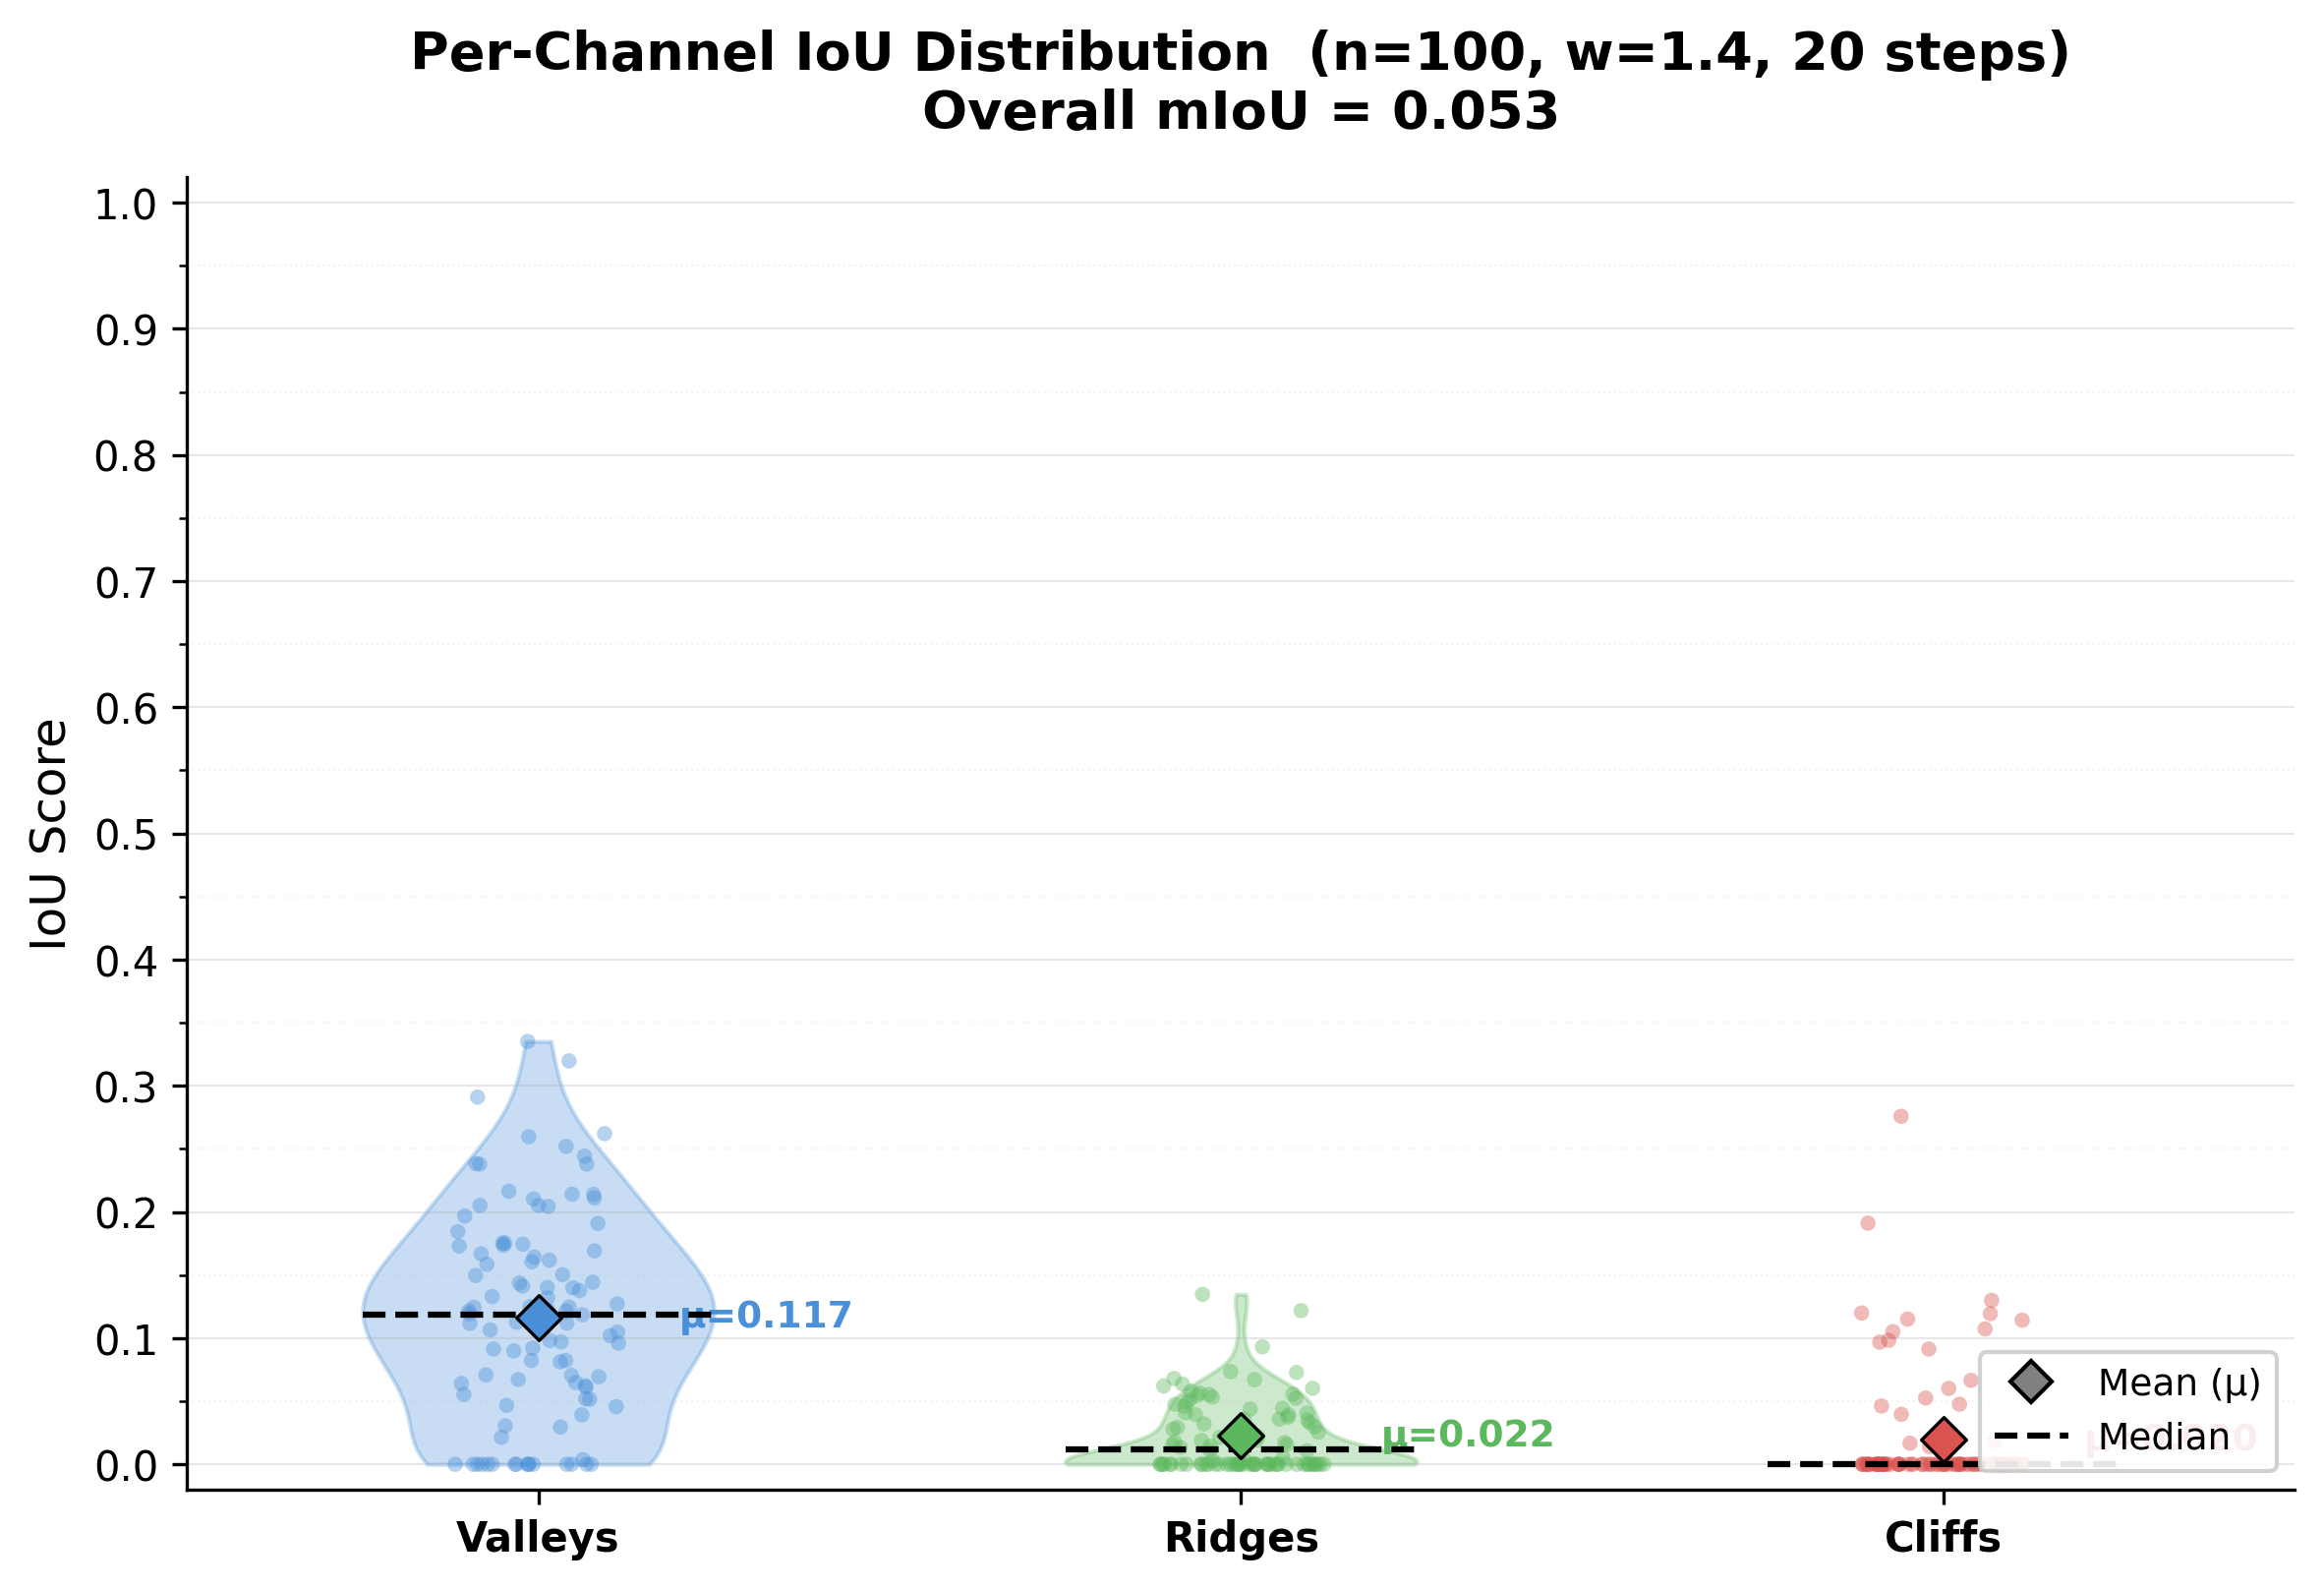
\includegraphics[width=0.85\linewidth]{images/iou_distribution.png}
	\caption{Per-channel Intersection over Union (IoU) distribution across 100 generated terrain samples with a control weight of $w = 1.4$. Each sample was produced by the trained ControlNet model using feature maps as conditioning hints. After generation, terrain features were re-extracted from the output DEM using the same feature extraction pipeline and compared against the original conditioning maps. The violin plots show the distribution of IoU scores per channel, with individual sample points overlaid as a strip plot. Diamond markers indicate the mean IoU per channel and dashed lines indicate the median.}
	\label{fig:iou_distribution}
\end{figure}

\subsection{Qualitative Analysis}
\label{sec:qualitative_analysis}

The qualitative comparison of generated satellite imagery across different control weights $w$ and conditioning maps is shown in Figure~\ref{fig:qualitative_comparison} and Figure~\ref{fig:qualitative_comparison_dem}. At $w = 0.0$, the model receives no conditioning signal and produces purely text-guided outputs, which exhibit a high degree of visual quality but lack alignment with the intended terrain features. The samples with higher $w$ show an increase in alignment with the conditioning maps, however, as $w$ increases, there is a noticeable decrease in visual quality, with higher weights leading to the overall image decreasing in visual quality.

\begin{figure}[htbp]
	\centering
	\includegraphics[width=\linewidth]{images/qualitative_comparison.png}
	\caption{Qualitative comparison of generated satellite imagery across different control weights $w$ and conditioning maps.}
	\label{fig:qualitative_comparison}
\end{figure}

\begin{figure}[htbp]
	\centering
	\includegraphics[width=\linewidth]{images/qualitative_comparison_dem.png}
	\caption{Qualitative comparison of generated DEM maps across different control weights $w$ and conditioning maps.}
	\label{fig:qualitative_comparison_dem}
\end{figure}


\subsection{Training Data Normalization}
\label{sec:training_data_normalization}

One potential explanation for the observed quality degradation of the generated landscapes at higher control weights is a mismatch in the training data distribution compared to the original training data of the pretrained model. For this training run the DEMs used for training were normalized to a $[-1,~1]$ range based on local maxima, while the pretrained model may have been trained on a different range. This discrepancy in data distribution can lead to difficulties in learning, as the model may struggle to adapt to the new input characteristics.

To investigate this hypothesis, a comparison of the training data distribution and the distribution of samples generated by the model was conducted. For easier comparison, the generated data and training data was mapped from $[-1,~1]$ to $[0,~1]$. The results indicate that the training data distribution of the normalized DEMs is indeed different from the original training data distribution of the pretrained model. The generated samples show a distribution around 0.5, while the training data distribution centers around 0.0 for RGB samples. For DEM samples, the center of the distribution is more similar, with 0.4 for training data and 0.5 for generated samples; however, the training data distribution is much more spread out across the whole range from 0 to 1, while the generated samples show a much narrower distribution around the center. This suggests that the model is struggling to learn the new data distribution, which may be contributing to the degradation of the outputs.


\begin{figure}[htbp]
	\centering
	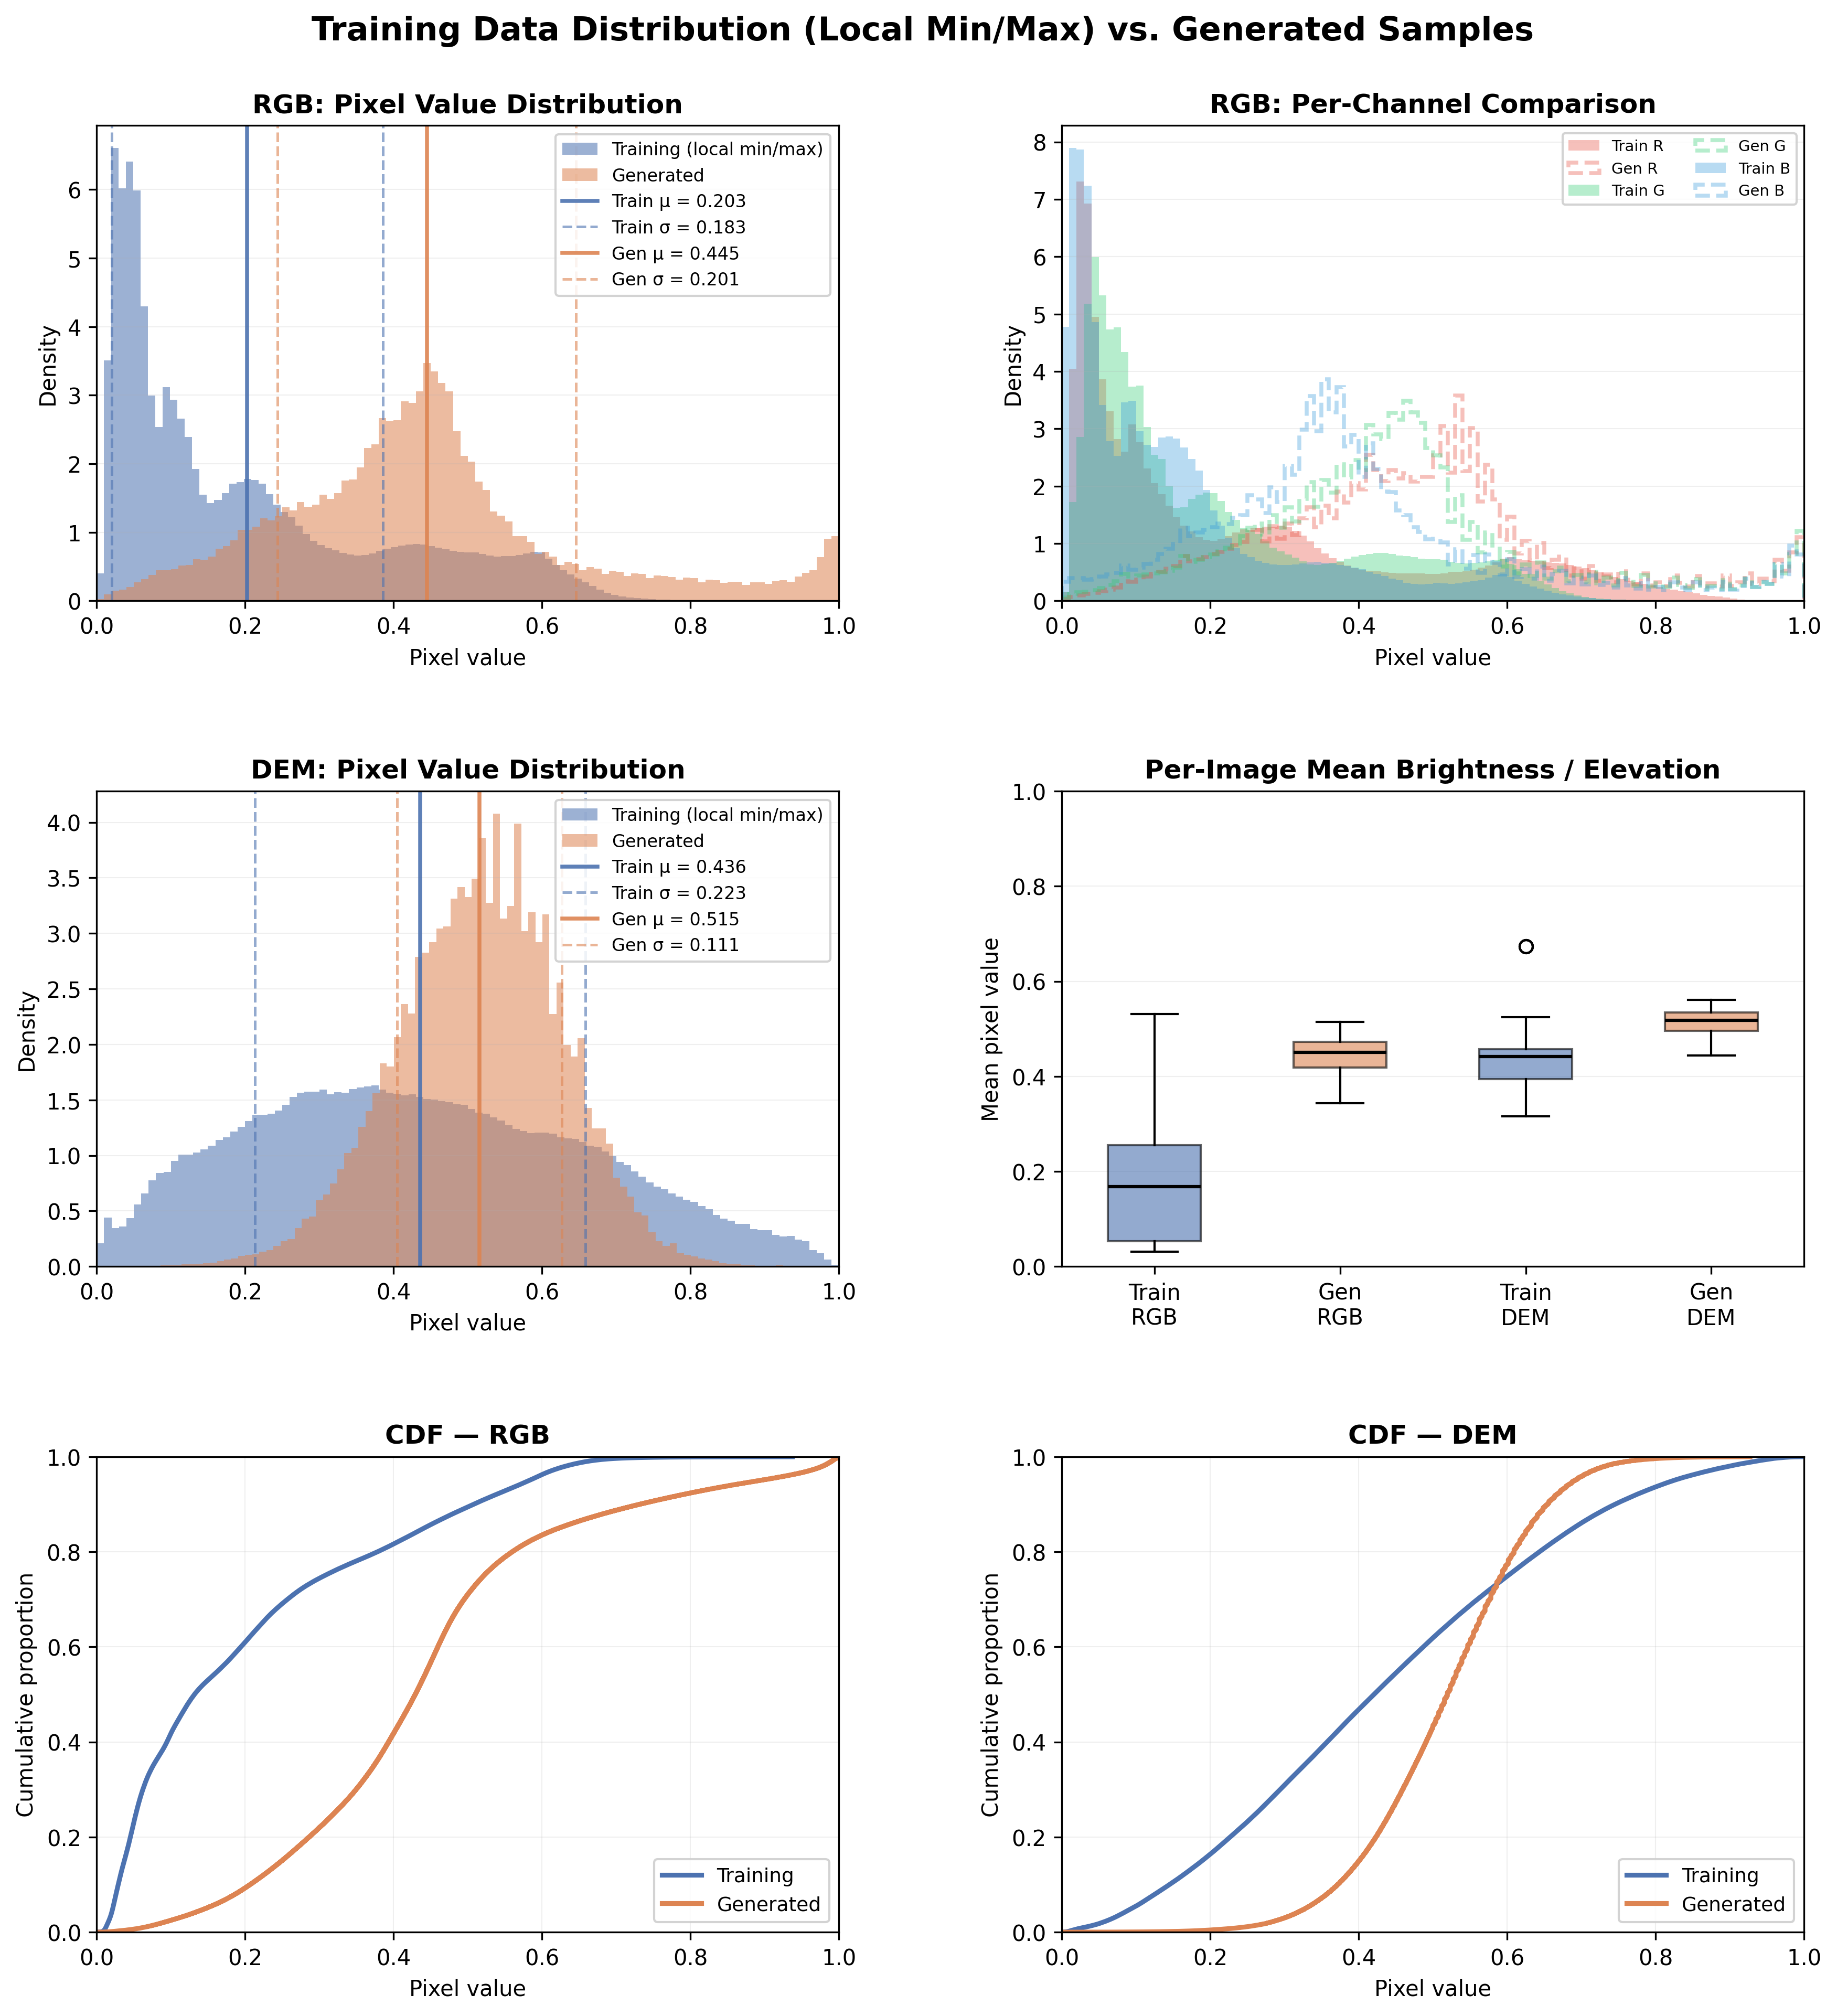
\includegraphics[width=\linewidth]{images/distribution_compare.png}
	\caption{Pixel-value distribution comparison between training data and model-generated samples across 50 images. \textbf{Row~1:} RGB histograms with mean~($\mu$) and standard deviation~($\sigma$) indicators, a per-channel breakdown. \textbf{Row~2:} DEM histograms with the same indicators, a box plot of per-image mean brightness and elevation. \textbf{Row~3:} CDF for both RGB and DEM pixel values.}
	\label{fig:distribution_compare}
\end{figure}

\section{Second Training Run}
\label{sec:second_training_run}

\subsection{Mitigating Data Distribution Mismatch}
\label{subsec:mitigating_data_distribution_mismatch}

To mitigate the data distribution mismatch, it is necessary to find a global normalization strategy that minimizes the distance between the training data distribution and the original training data distribution of the pretrained model. For this purpose Nelder-Mead~\cite{nelder1965simplex} optimization was employed to find the optimal $min$ and $max$ parameters that minimize the Wasserstein~\cite{villani2009optimal} distance between the training data distribution and a sample distribution generated by the model.

The comparison of the new training data distribution with the generated sample distribution, shown in Figure~\ref{fig:new_distribution_compare}, demonstrates that the global normalization strategy has improved the alignment between the training data and the generated samples compared to the previous local normalization approach. The DEM distributions now show a closer match between the training data and generated samples.

\begin{figure}[htbp]
	\centering
	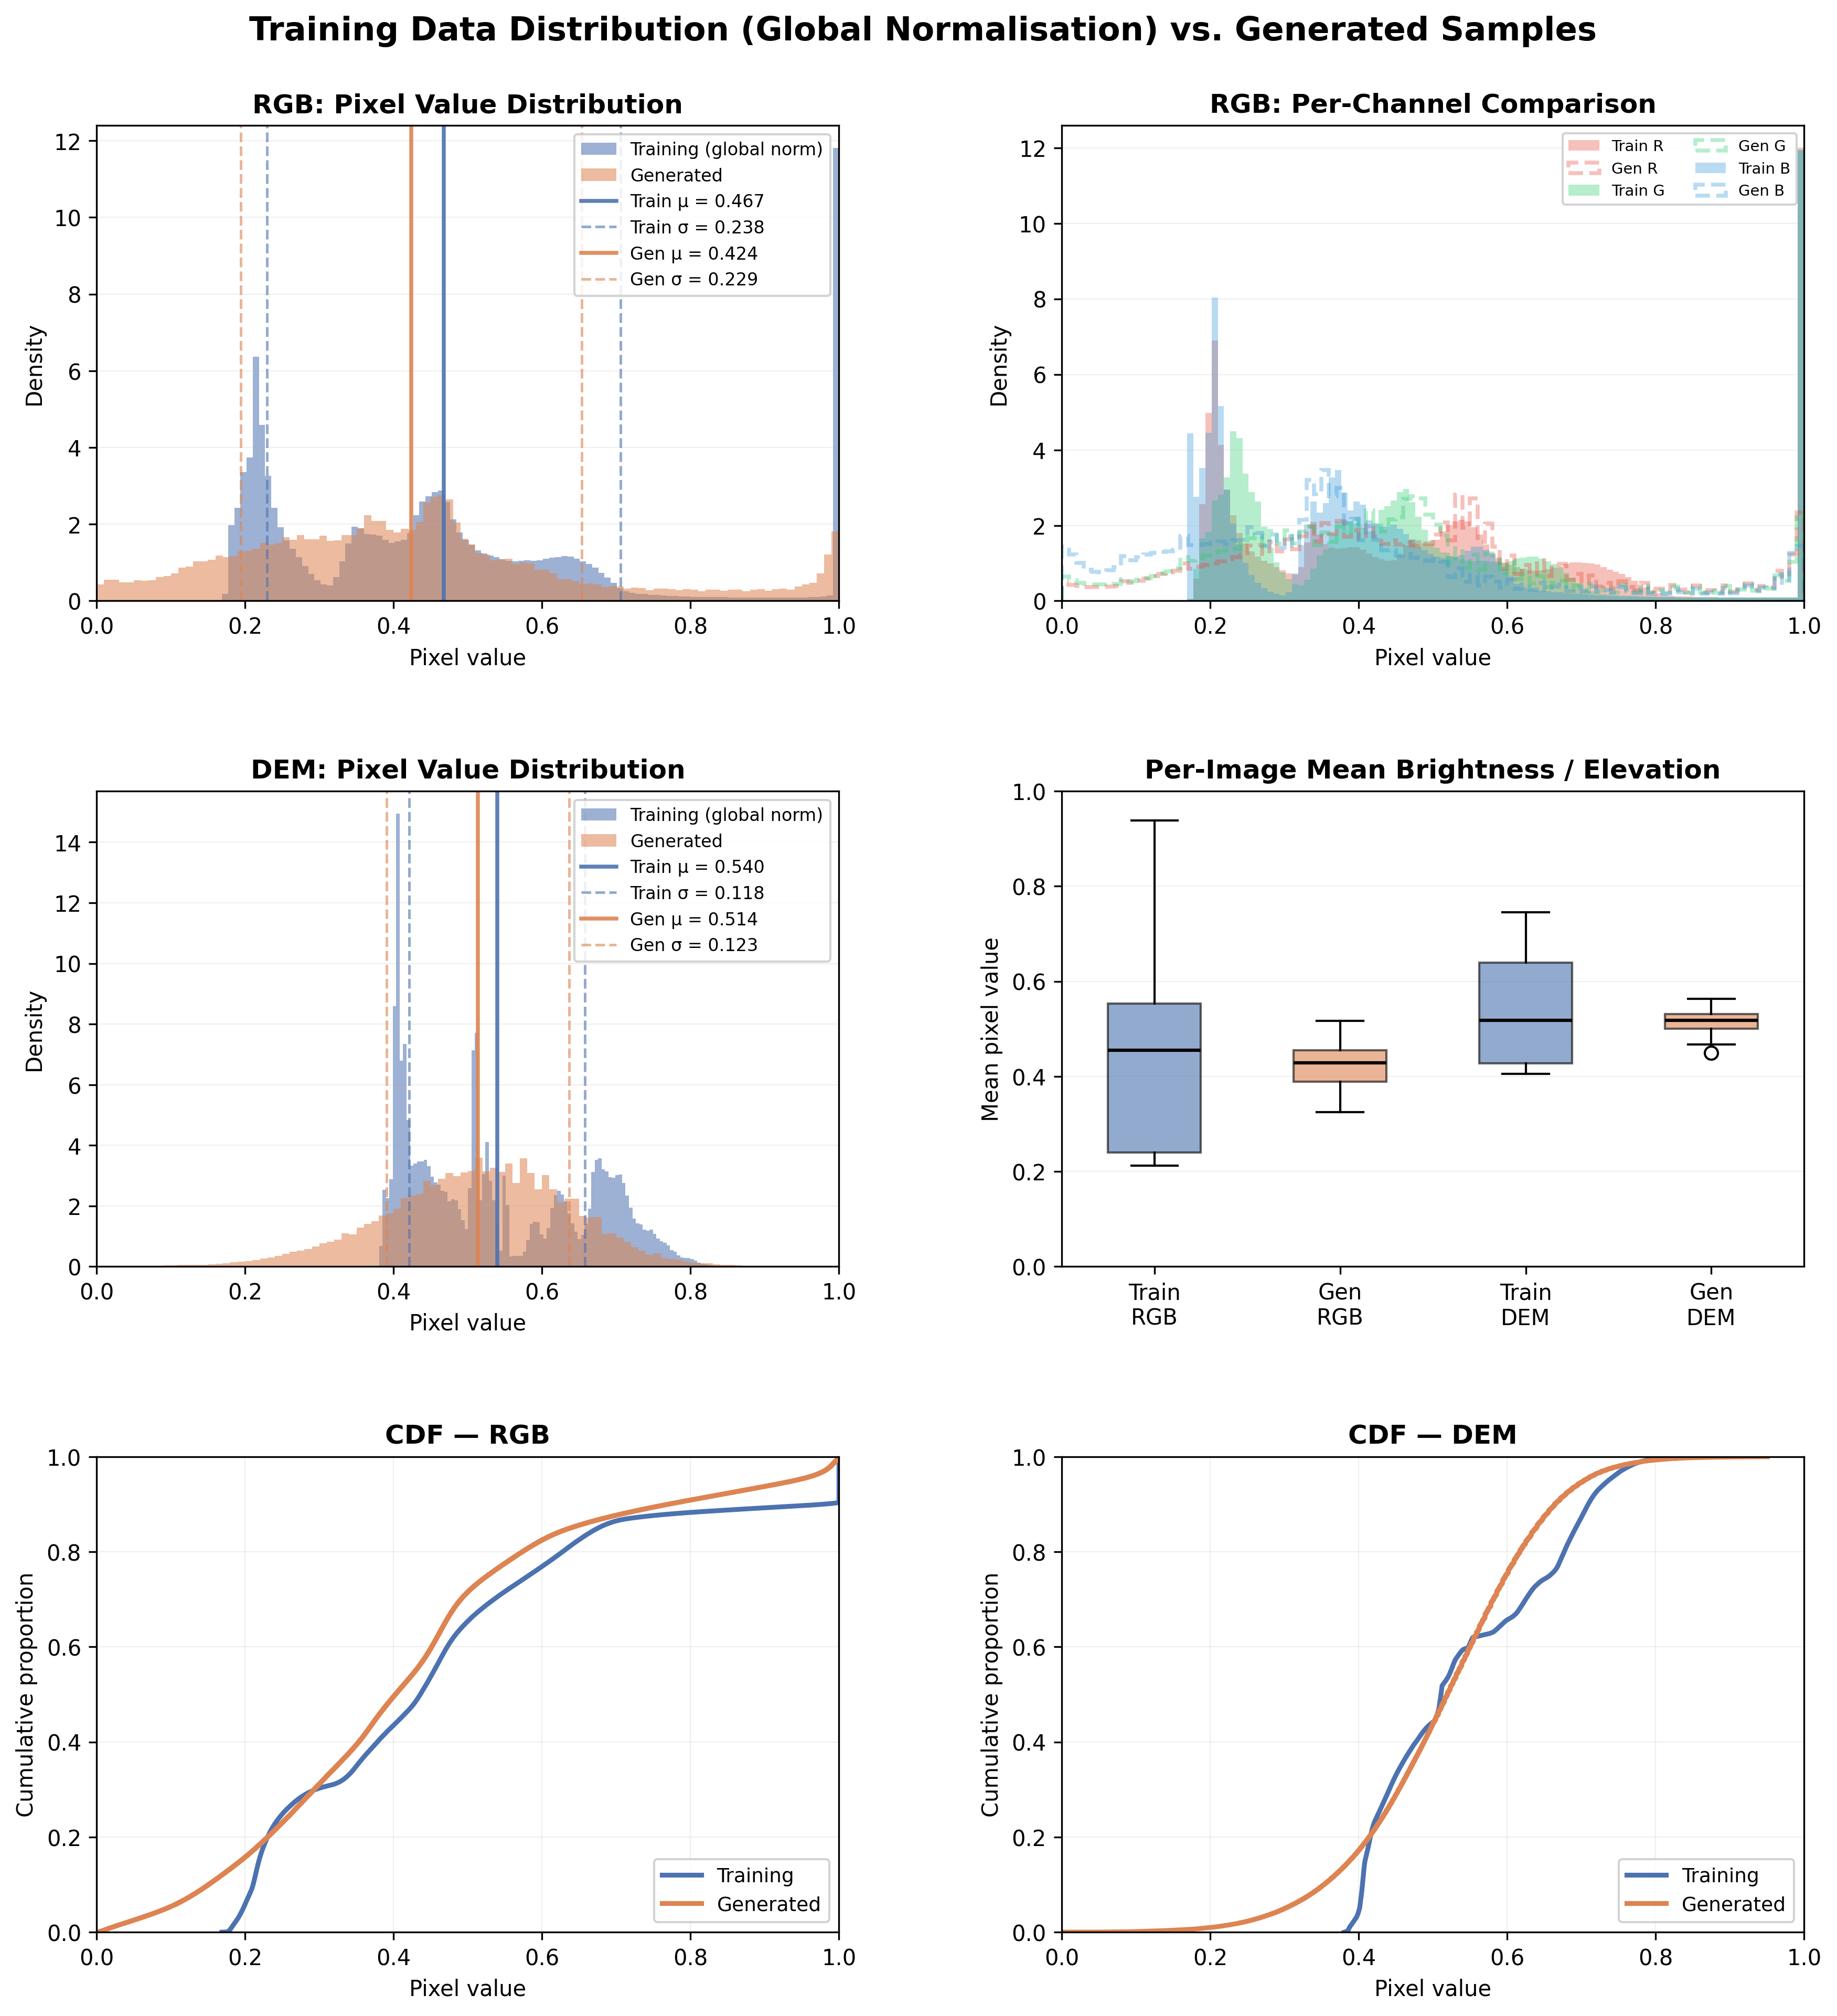
\includegraphics[width=\linewidth]{images/new_distribution_compare.png}
	\caption{Pixel-value distribution comparison between training data with global normalization and model-generated samples across 50 images. \textbf{Row~1:} RGB histograms with mean and standard deviation indicators, a per-channel breakdown. \textbf{Row~2:} DEM histograms with the same indicators, a box plot of per-image mean brightness and elevation. \textbf{Row~3:} CDF for both RGB and DEM pixel values.}
	\label{fig:new_distribution_compare}
\end{figure}

\subsection{Training on new normalization}
\label{subsec:training_on_new_normalization}

The training metrics for the second training run, shown in Figure~\ref{fig:new_training_metrics}, demonstrate improved training behavior compared to the first run. The training was conducted for a total of $40\,000$ steps using the Prodigy optimizer with fp16 precision and the new global normalization strategy.

\begin{figure}[htbp]
	\centering
	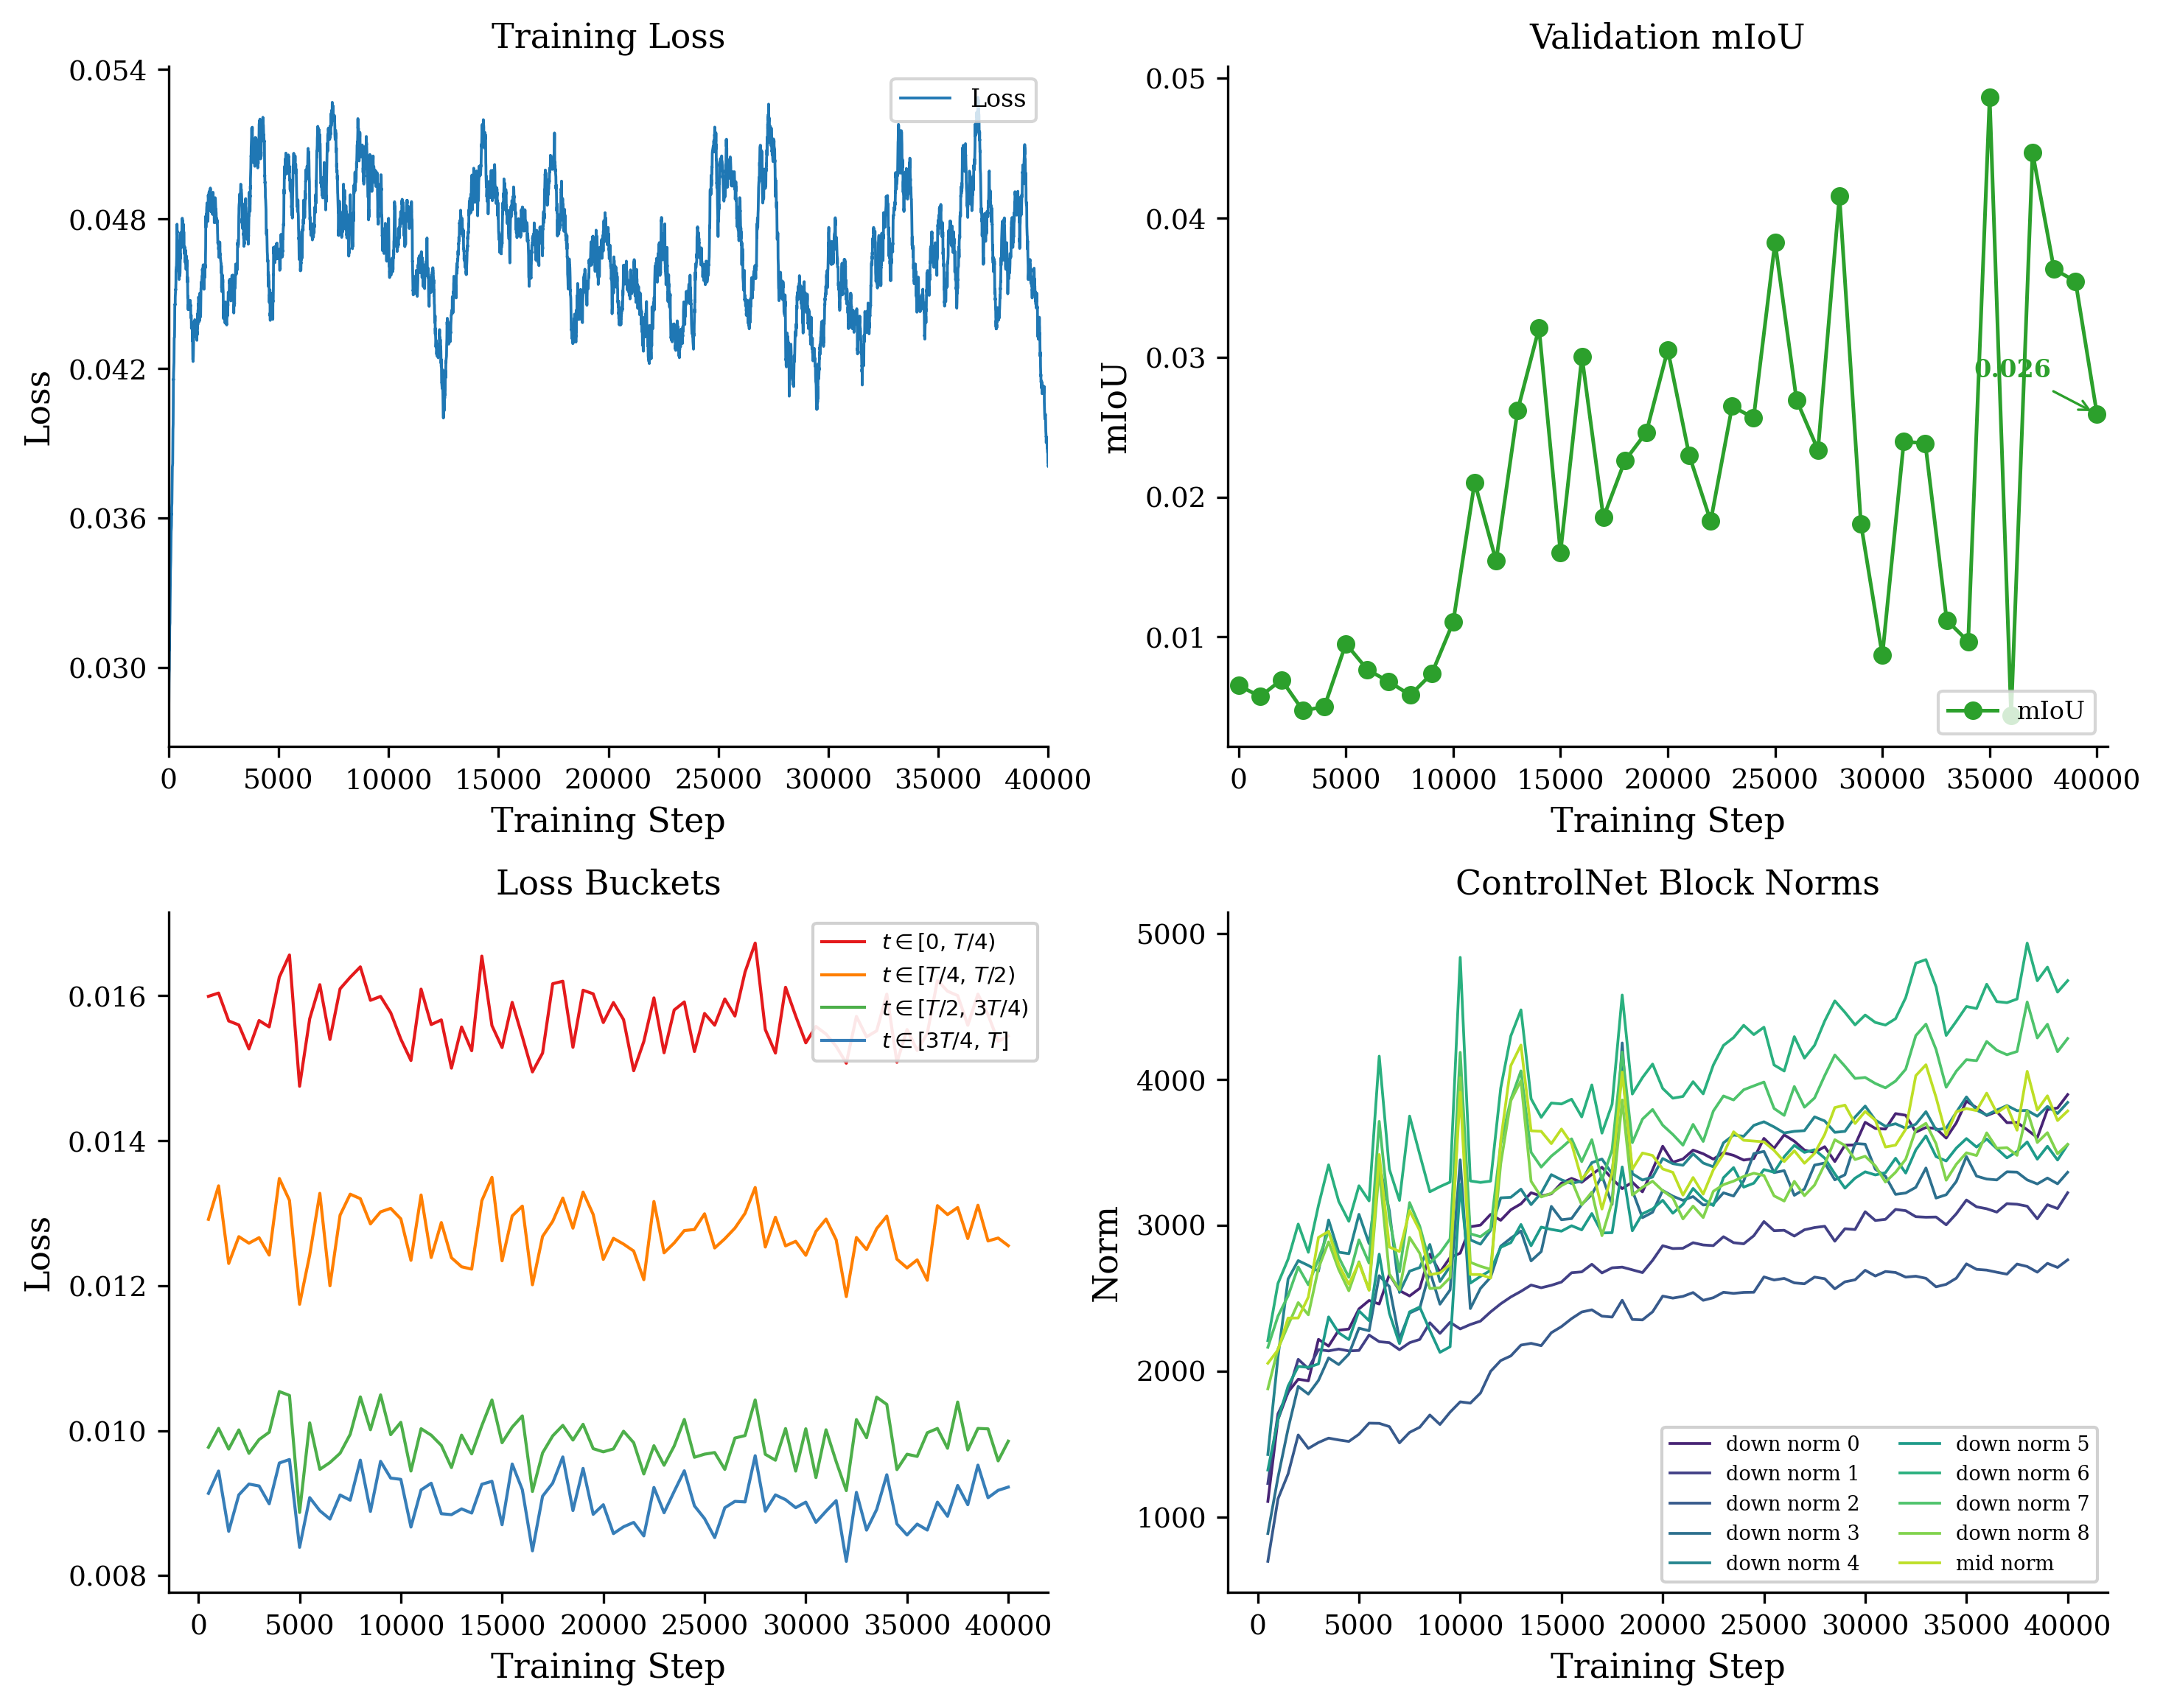
\includegraphics[width=\linewidth]{images/new_training_metrics.png}
	\caption{Training metrics for the second training run with the new normalization strategy. \textbf{Top-left:} training loss with a 200-step rolling average. \textbf{Top-right:} validation mean Intersection over Union evaluated every $1\,000$ steps. \textbf{Bottom-left:} per-bucket loss decomposed by noise level ($t/4$ quantiles). \textbf{Bottom-right:} norms of the ControlNet residual outputs per block.}
	\label{fig:new_training_metrics}
\end{figure}

\subsection{Qualitative Evaluation}
\label{subsec:evaluation2}

The qualitative comparison for the second training run, shown in Figure~\ref{fig:new_qualitative_comparison} and Figure~\ref{fig:new_qualitative_comparison_dem}, demonstrates the effect of varying the conditioning scale $w$ on the generated terrain using the model trained with the new normalization strategy. Compared to the first training run, the generated images maintain better visual quality at higher control weights, with less artifacts than previously observed. The model broadly follows the conditioning maps, with higher control weights leading to better alignment with the intended terrain features. However, there is still a noticeable decrease in visual quality at higher control weights, suggesting that while the new normalization strategy has improved the training process, there may still be challenges in achieving control while not degrading visual quality. Another issue is that the features besides valley show a lower degree of alignment with the conditioning maps, which is consistent with the quantitative evaluation results showing lower IoU for these features.

\begin{figure}[htbp]
	\centering
	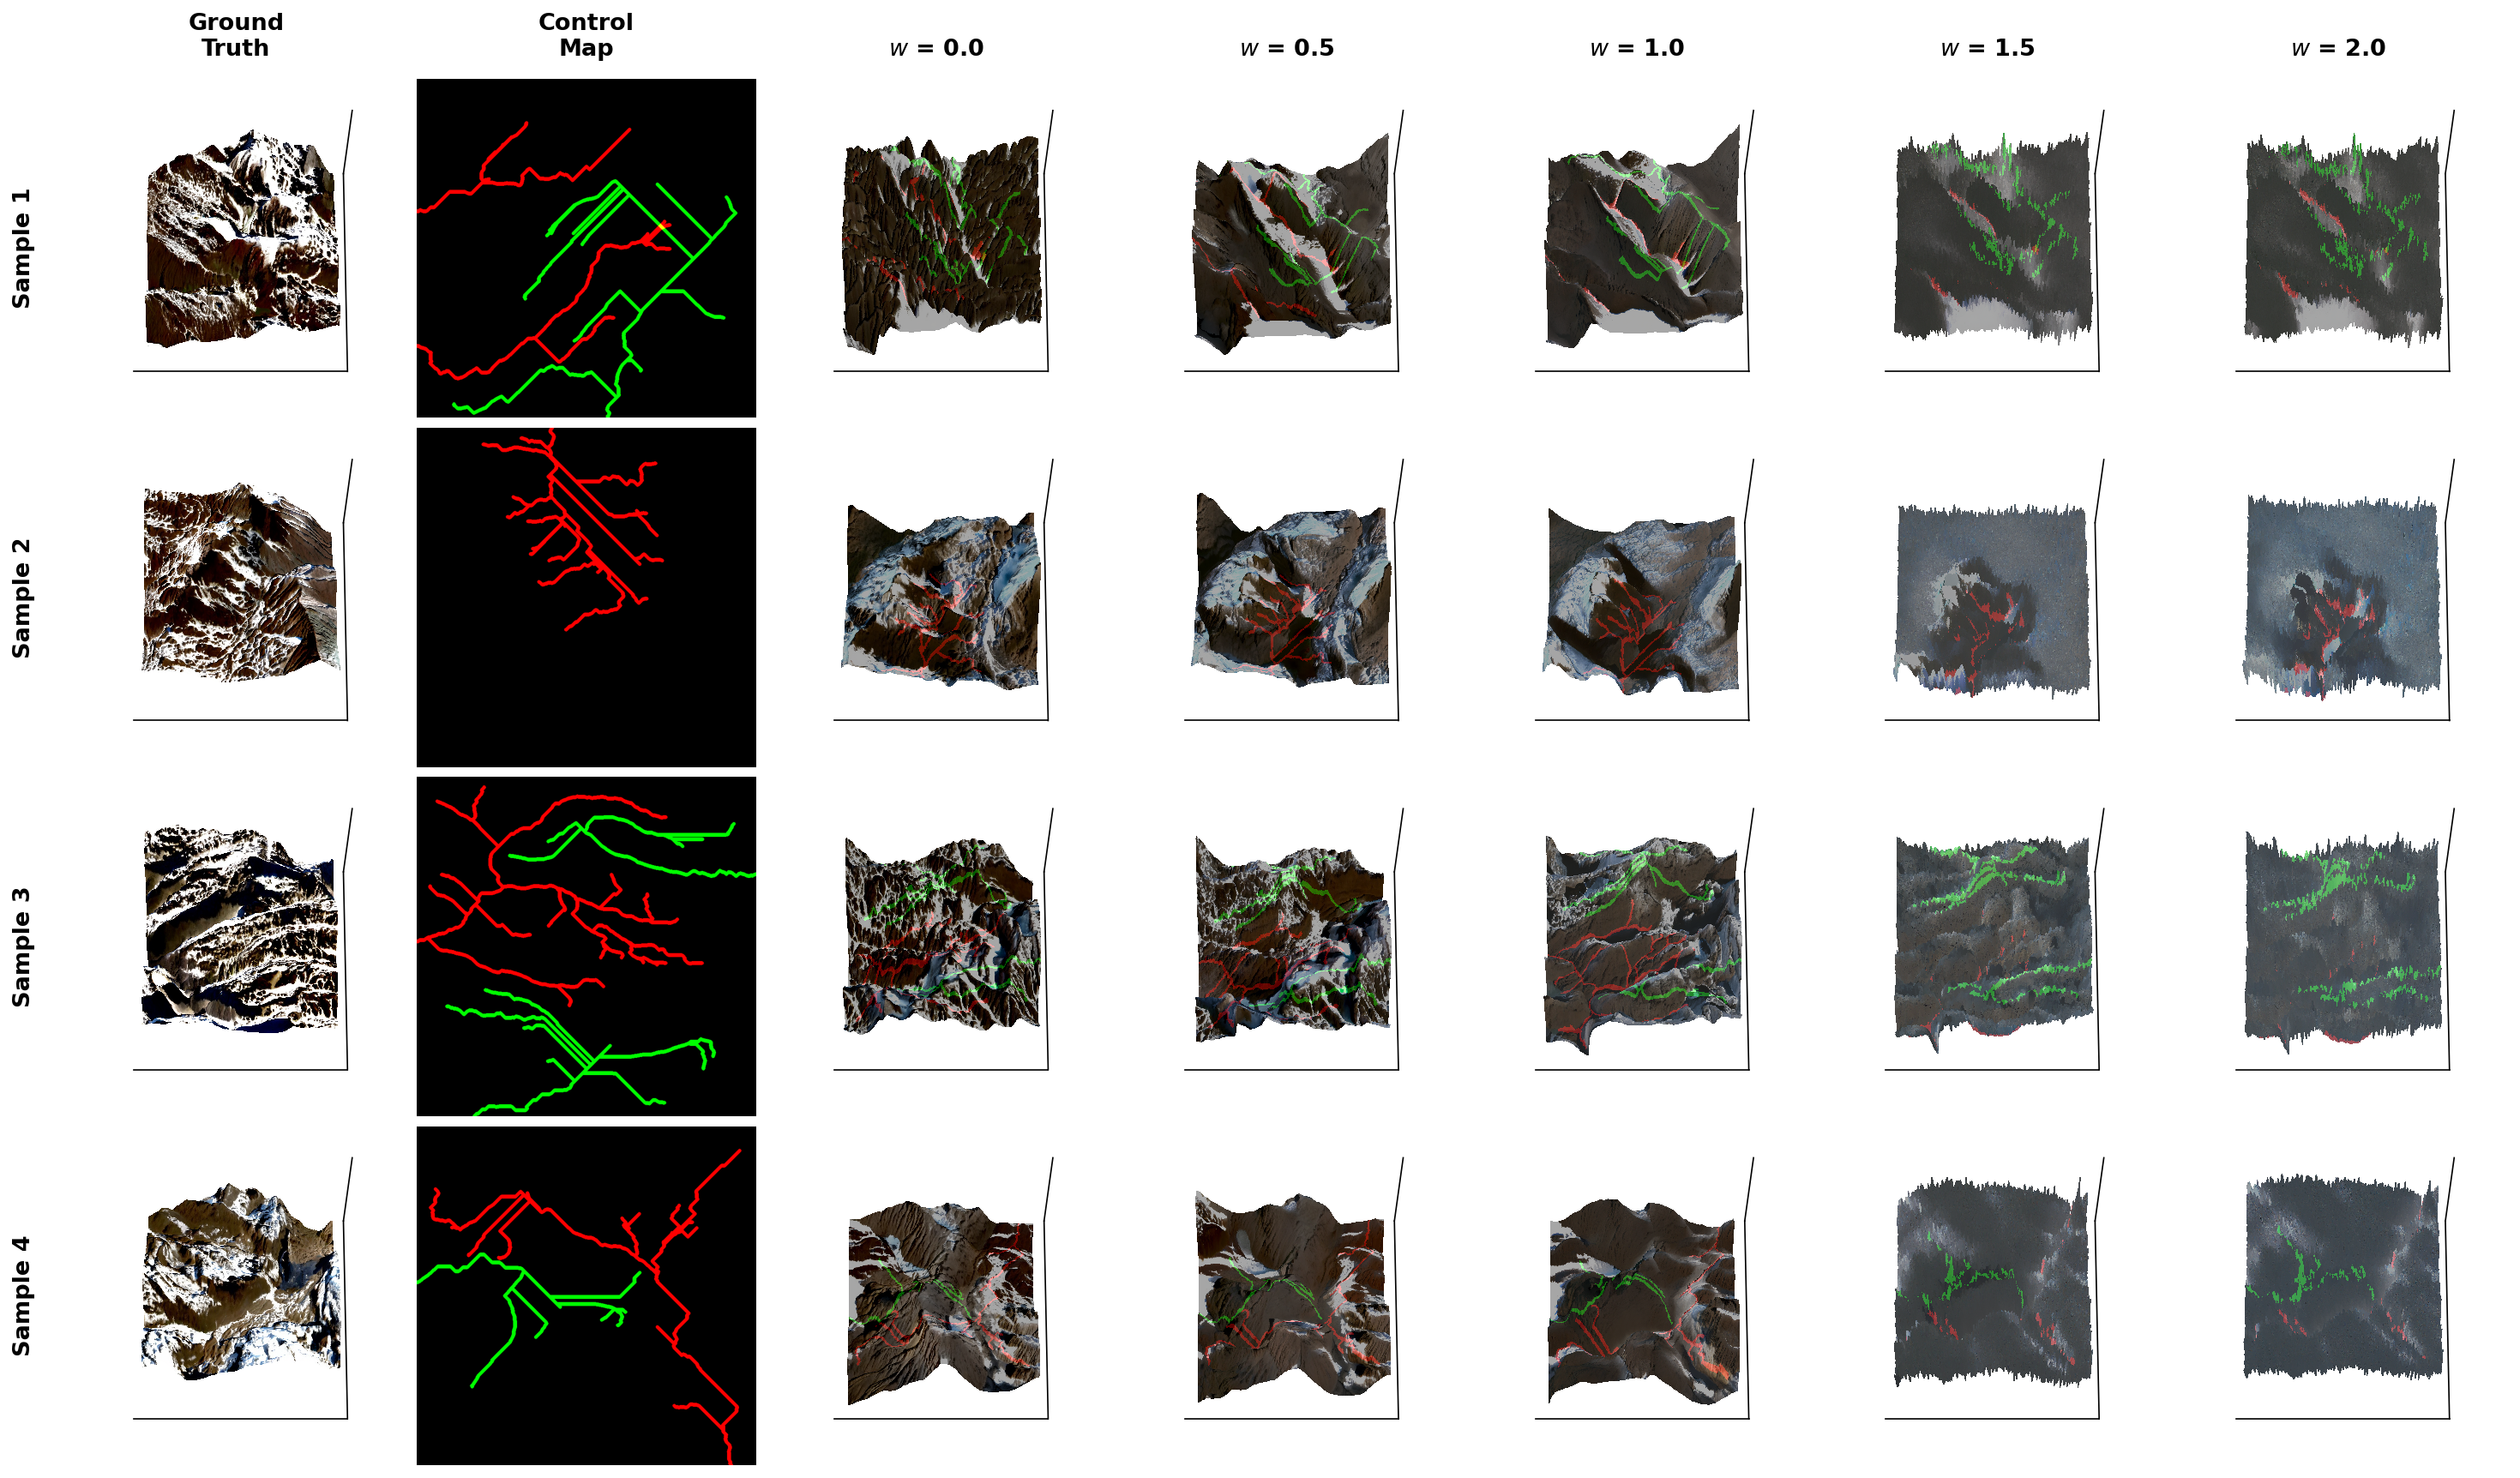
\includegraphics[width=\linewidth]{images/new_qualitative_comparison.png}
	\caption{Qualitative comparison of generated satellite imagery across different control weights $w$ and conditioning maps for the second training run with the new normalization strategy.}
	\label{fig:new_qualitative_comparison}
\end{figure}
\begin{figure}[htbp]
	\centering
	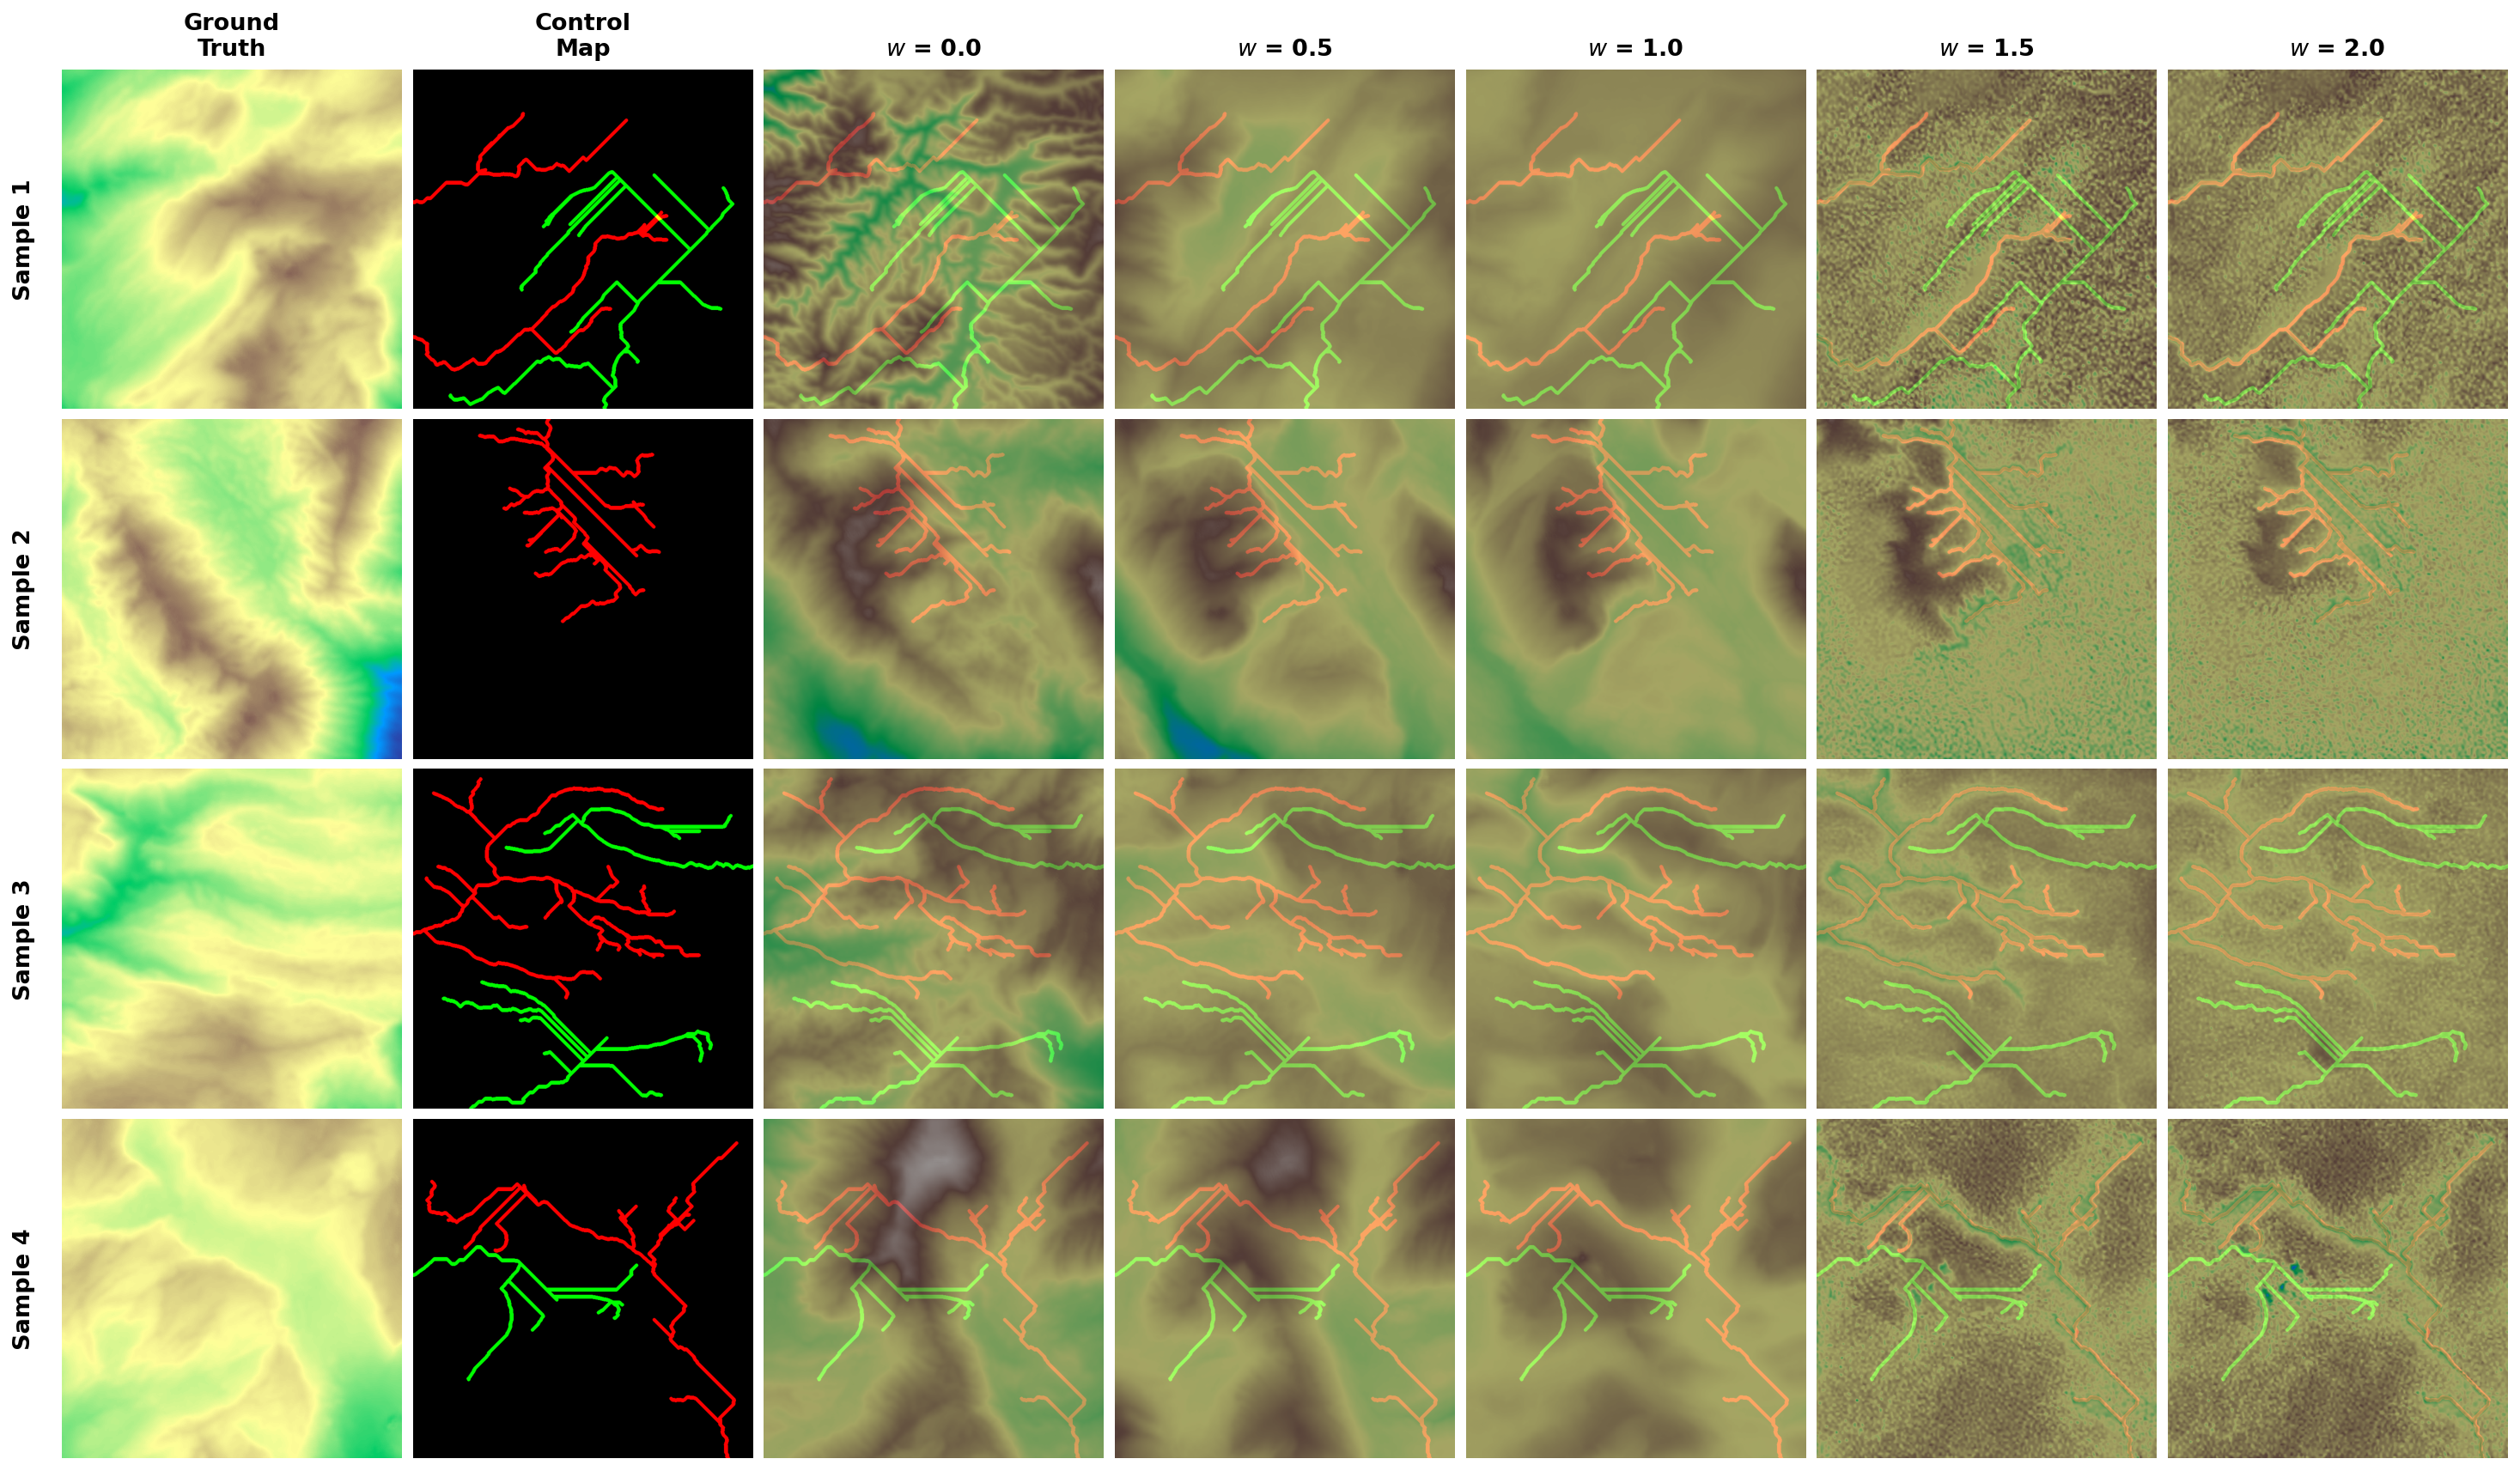
\includegraphics[width=\linewidth]{images/new_qualitative_comparison_dem.png}
	\caption{Qualitative comparison of generated DEM maps across different control weights $w$ and conditioning maps.}
	\label{fig:new_qualitative_comparison_dem}
\end{figure}

\subsection{Quantitative Evaluation}
\label{subsec:quantitative_evaluation2}


The quantitative evaluation of the second training run, shown in Figure~\ref{fig:new_iou_distribution}, presents the per-channel IoU distribution across 100 generated terrain samples with a control weight of $w = 1.4$. The results show an improvement in the mean IoU for ridges and cliffs compared to the first training run, but the mean IoU for valleys has decreased on average compared to the first run. The variance of IoU scores remains high for all channels, which may still be attributed to the model being undertrained or due to the sensitivity of the IoU metric to small misalignments in the feature maps. Overall, while there is some improvement in alignment with the conditioning maps, there is still room for further optimization and training to achieve more consistent results across all terrain features.

\begin{figure}[htbp]
	\centering
	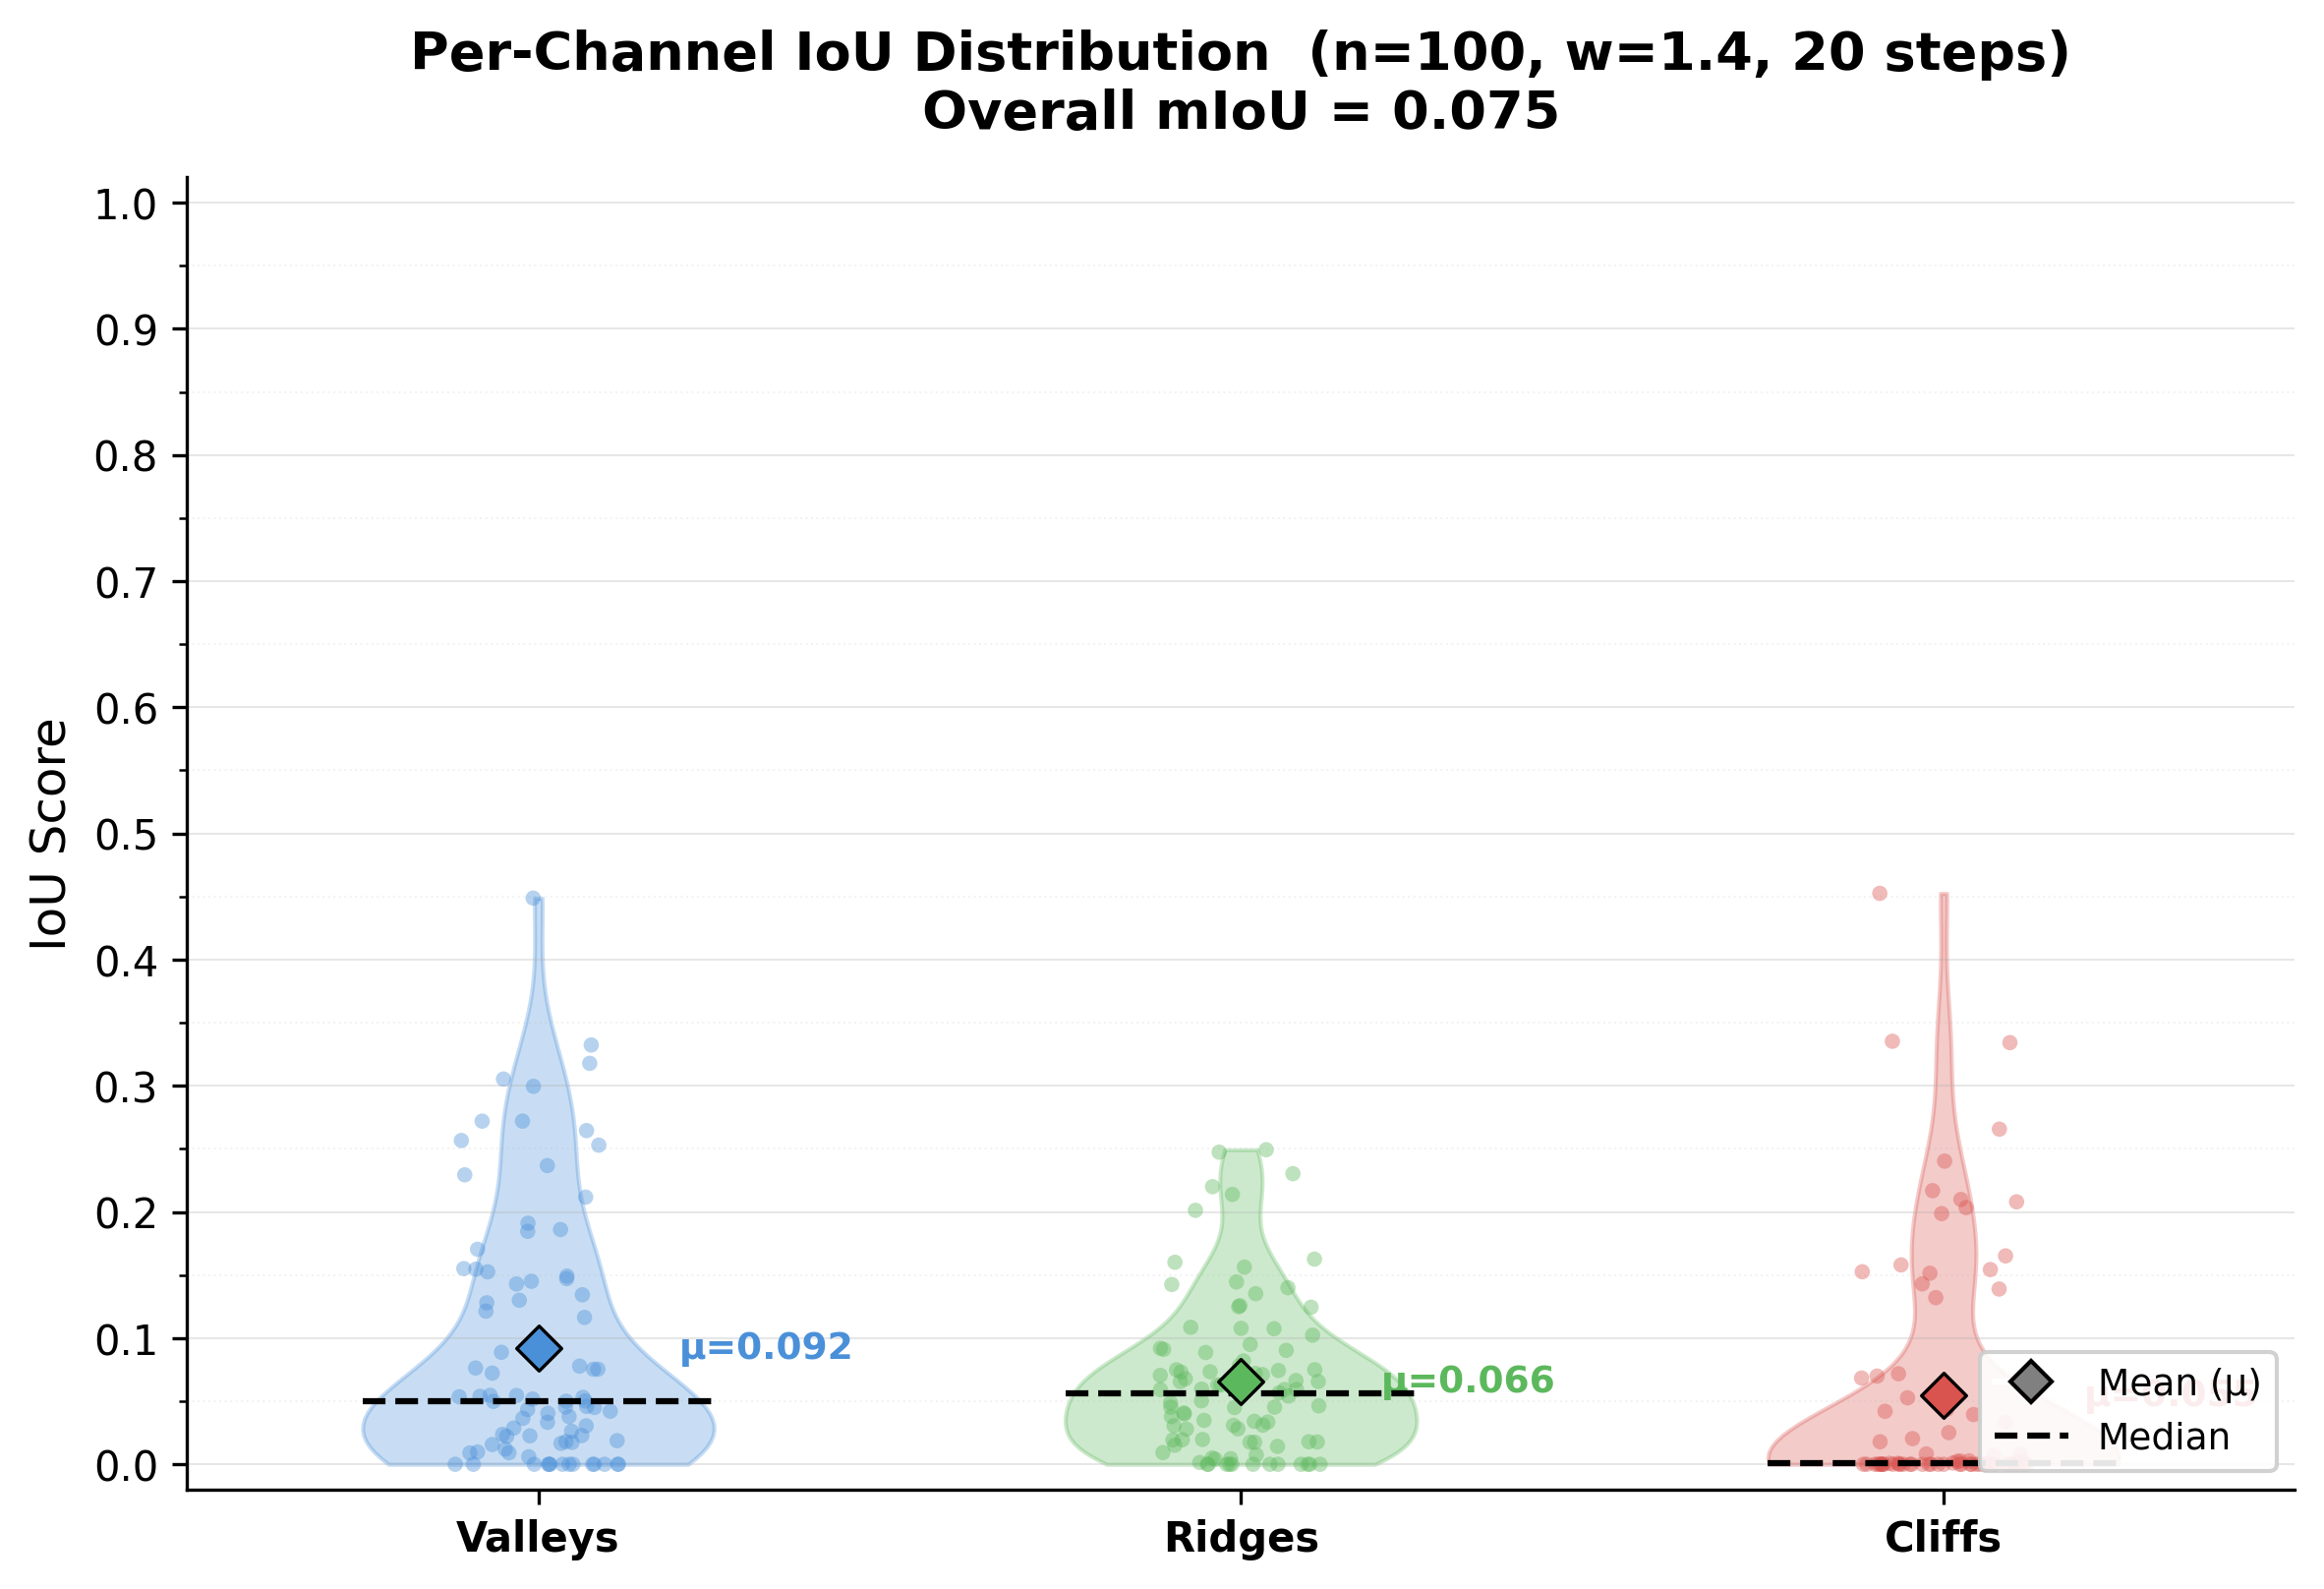
\includegraphics[width=0.85\linewidth]{images/new_iou_distribution.png}
	\caption{Per-channel Intersection over Union (IoU) distribution across 100 generated terrain samples with a control weight of $w = 1.4$ for the second training run with the new normalization strategy. The violin plots show the distribution of IoU scores per channel, with individual sample points overlaid as a strip plot. Diamond markers indicate the mean IoU ($\mu$) per channel and dashed lines indicate the median.}
	\label{fig:new_iou_distribution}
\end{figure}


\subsection{Results on synthetic feature maps}
\label{subsec:results_on_synthetic_feature_maps}

To further evaluate the model's ability to learn spatial conditioning, a set of synthetic feature maps with simple geometric patterns was created and used as conditioning inputs for generation. The results, shown in Figure~\ref{fig:synthetic_feature_maps}, demonstrate that the model is able to generate landscapes that follow the structure of the synthetic conditioning maps in most cases, with the generated DEMs and satellite images showing alignment with the intended patterns. However, there are some cases where the conditioning has little impact, especially on images with only ridges or cliffs, which is consistent with the quantitative evaluation results showing lower IoU for these features. When the feature map is too far removed from plausible real-world terrain, the model struggles to generate meaningful outputs. Overall, the results on synthetic feature maps provide additional evidence that the model has learned to some extent to utilize the spatial conditioning, but there are still limitations in terms of the consistency and strength of the conditioning effect across different terrain features and patterns.

\begin{figure}[htbp]
	\centering
	\includegraphics[width=0.85\linewidth]{images/synthetic_conditioning.png}
	\caption{Generation conditioned on synthetic feature maps. \textbf{First Column:} synthetic conditioning maps with a simple geometric pattern. \textbf{Second Column:} generated DEM. \textbf{Third Column:} generated satellite image. \textbf{Fourth Column:} 3D visualization of the generated terrain.}
	\label{fig:synthetic_feature_maps}
\end{figure}
